\documentclass[12pt, a4paper]{report}

% --- Carreguem el preàmbul ---
% --- Paquets fonamentals ---
\usepackage[utf8]{inputenc}
\usepackage[T1]{fontenc}
\usepackage[catalan]{babel}
\usepackage{graphicx}
\usepackage{float}
\usepackage{setspace}
\usepackage{geometry}
\usepackage{xcolor}
\usepackage{titlesec}
\usepackage{fancyhdr}
\usepackage{tocloft}
\usepackage{enumitem}
\usepackage{hyperref} % Hipervíncles
\usepackage{tikz}     % Diagrames
\usetikzlibrary{arrows.meta, positioning, shapes.geometric}
\usepackage{listings} % Codi font
\usepackage{caption}  % Peus de figura millorats
\usepackage{booktabs} % Taules professionals

% --- Font Formal (Tipus Arial/Helvetica per a TDR) ---
\usepackage{helvet}
\renewcommand{\familydefault}{\sfdefault}

% --- Configuració de Marges ---
\geometry{a4paper, margin=2.5cm, headheight=20pt, footskip=1.5cm} 

% --- Configuració d'Espaiat ---
\onehalfspacing 

% --- Definició de Colors Sobris i Moderns ---
\definecolor{DarkBlue}{RGB}{0, 51, 102}
\definecolor{SoftGray}{RGB}{245, 245, 245}
\definecolor{HeaderGray}{RGB}{80, 80, 80}

% --- Configuració de hyperref ---
\hypersetup{
    colorlinks=true,
    linkcolor=DarkBlue,
    filecolor=magenta,      
    urlcolor=DarkBlue,
    citecolor=DarkBlue,
}

% --- Estil de Títols ---
\titleformat{\chapter}[hang]
  {\normalfont\huge\bfseries\color{DarkBlue}}
  {\thechapter.}{1em}{}
\titlespacing*{\chapter}{0pt}{-20pt}{20pt}

\titleformat{\section}{\color{DarkBlue}\Large\bfseries}{\thesection.}{1em}{}
\titlespacing*{\section}{0pt}{12pt}{6pt}

\titleformat{\subsection}{\color{DarkBlue}\large\bfseries}{\thesubsection.}{1em}{}
\titlespacing*{\subsection}{0pt}{10pt}{4pt}

% Activar numeració fins a subseccions
\setcounter{secnumdepth}{3}
\setcounter{tocdepth}{2}

% --- Configuració de Capçaleres i Peus ---
\pagestyle{fancy}
\fancyhf{}
\lhead{\small\color{HeaderGray} IE Sant Pol de Mar}
\rhead{\small\color{HeaderGray}\nouppercase{\leftmark}}
\lfoot{\small\color{HeaderGray} Genís Olivé Fernández}
\rfoot{\small\color{HeaderGray} Pàgina \thepage}
\renewcommand{\headrulewidth}{0.4pt}
\renewcommand{\footrulewidth}{0.4pt}

% Forçar estil en pàgines de capítol (plain)
\fancypagestyle{plain}{
    \fancyhf{}
    \lhead{\small\color{HeaderGray} IE Sant Pol de Mar}
    \rhead{\small\color{HeaderGray}\nouppercase{\leftmark}}
    \lfoot{\small\color{HeaderGray} Genís Olivé Fernández}
    \rfoot{\small\color{HeaderGray} Pàgina \thepage}
    \renewcommand{\headrulewidth}{0.4pt}
    \renewcommand{\footrulewidth}{0.4pt}
}

% --- Configuració de listings (Codi Python) ---
\lstset{
    backgroundcolor=\color{SoftGray},   
    commentstyle=\color{green!60!black},
    keywordstyle=\color{DarkBlue},
    numberstyle=\tiny\color{HeaderGray},
    stringstyle=\color{orange},
    basicstyle=\ttfamily\small,
    breakatwhitespace=false,         
    breaklines=true,                 
    captionpos=b,                    
    keepspaces=true,                 
    numbers=left,                    
    numbersep=5pt,                  
    showspaces=false,                
    showstringspaces=false,
    showtabs=false,                  
    tabsize=2,
    frame=single,
    rulecolor=\color{DarkBlue!30}
}

% --- Índex ---
\renewcommand{\cfttoctitlefont}{\Huge\bfseries\color{DarkBlue}}
\renewcommand{\cftchapfont}{\bfseries\color{DarkBlue}}


\begin{document}

% --- Portada ---
\begin{titlepage}
    \centering
    \vspace*{-2cm}
    
    
\includegraphics[height=1.8cm]{images/logo-institut.png} \\
    \vspace{0.5cm}
    {\large \textbf{IE Sant Pol de Mar}} \\
    \vspace{2.5cm}

    {\huge \bfseries \color{DarkBlue} Poden les veles rígides reduir el consum de combustible en els vaixells de gran eslora? \par}
    \vspace{1.5cm}

    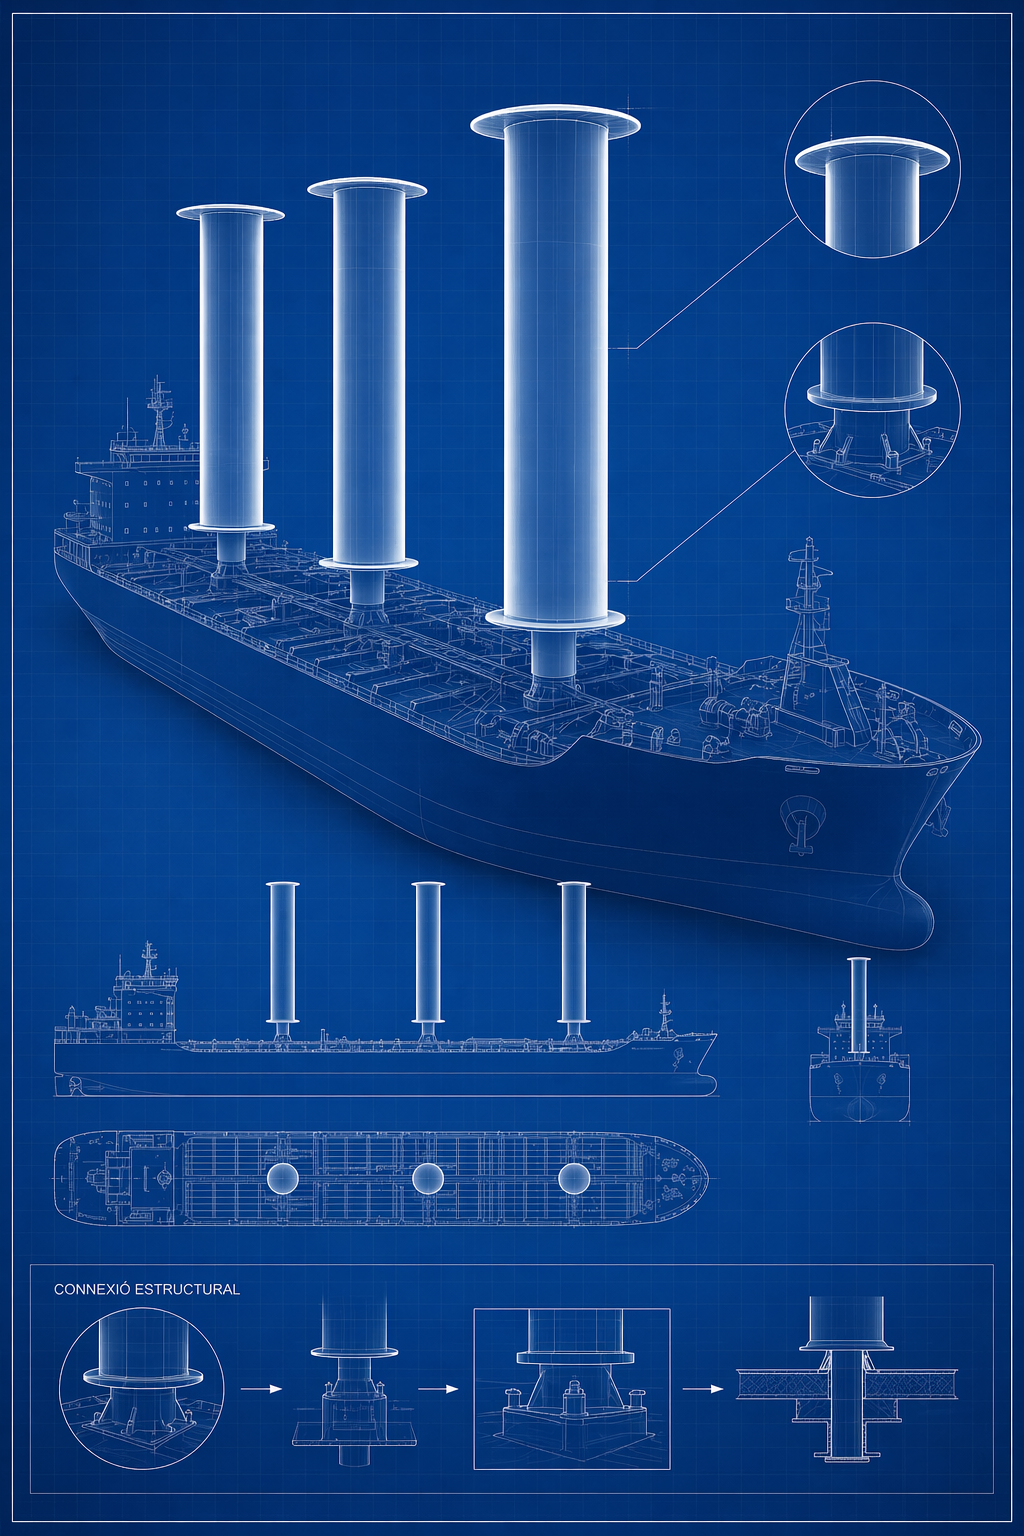
\includegraphics[width=0.75\textwidth]{images/imatge-portada.png} \\
    \vspace{0.2cm}
    {\footnotesize \textit{Visualització d'un mercant modern amb propulsió eòlica rígida.}} 

    \vfill

    \begin{minipage}{0.45\textwidth}
        \begin{flushleft} \large
            \textbf{Autor:}\\
            Genís Olivé Fernández
        \end{flushleft}
    \end{minipage}
    \begin{minipage}{0.45\textwidth}
        \begin{flushright} \large
            \textbf{Tutor:}\\
            Arnau Pou Raurell
        \end{flushright}
    \end{minipage}

    \vspace{1.5cm}
    {\large \textbf{Curs 2025-2026}} \\
    \vspace{0.5cm}
    {\small Treball de Recerca de Batxillerat}
\end{titlepage}

% --- Índex ---
\newpage
\vspace*{-1.5cm}
\tableofcontents
\clearpage

% --- Seccions del Treball ---
\pagenumbering{arabic}
\chapter*{Resum}
\addcontentsline{toc}{chapter}{Resum}

Aquest Treball de Recerca investiga la viabilitat de les veles rígides com a sistema de propulsió auxiliar per reduir el consum de combustible i les emissions de $CO_2$ en els vaixells de gran eslora. A través de l'estudi dels fonaments aerodinàmics i l'anàlisi de dades de simulació, es demostra que aquesta tecnologia pot generar estalvis d'entre el 15\% i el 30\%, depenent de les rutes i les condicions meteorològiques.

\vspace{1cm}

\chapter*{Abstract}
\addcontentsline{toc}{chapter}{Abstract}

This Research Project investigates the feasibility of wing sails as an auxiliary propulsion system to reduce fuel consumption and $CO_2$ emissions in large ships. Through the study of aerodynamic foundations and the analysis of simulation data, it is shown that this technology can generate savings between 15\% and 30\%, depending on routes and weather conditions.

\chapter*{Introducció}
\addcontentsline{toc}{chapter}{Introducció}

\section*{Motivació i justificació del tema}
% Text de la motivació...
Aquest treball de recerca parteix de la necessitat de poder crear una alternativa més sostenible per reduir el consum de combustible en els vaixells dins del sector del comerç marítim arreu del món, 
ja que aquest representa vora un 90\% del transport de mercaderies globalment. 
D'aquesta manera, que si aconseguíssim fer aquest canvi per rebaixar el combustible utilitzat, suposaria un estalvi immens. 
A més, com que el combustible és finit, no podrem dependre sempre d'aquesta font d'energia. 
Per aquest motiu, aquest treball pretén mostrar una alternativa sostenible i reutilitzable.
\section*{Objectius de la recerca}
% Text dels objectius...
Un dels objectius de fer aquest projecte és poder analitzar com funcionen els diferents sistemes de propulsió marítima per als vaixells 
i comparar-los per veure quins són més adequats en cada context.
\section*{Hipòtesi}
% Text de la hipòtesi...
La hipòtesi que es planteja en aquest projecte, es preveu que els resultats d'analitzar 
aquestes tecnologies comparades amb altres sistemes de propulsió presentin un millor rendiment
en termes d'eficiència i cost econòmic a llarg termini. 
Respecte a la maqueta, es preveu que representarà correctament el funcionament 
de la propulsió, però que segurament es veurà afectada l'eficiència 
a falta de condicions reals.
\section*{Metodologia}
% Text de la metodologia...

\chapter{Objectius i Hipòtesi}
\section{Objectius}
% Llista aquí els teus objectius...

\section{Hipòtesi}
% Descriu la teva hipòtesi de recerca...

\chapter{Fonaments físics i aerodinàmics}
\section{Principis d'aerodinàmica: Sustentació (Lift) i Arrossegament (Drag)}

El funcionament de les veles rígides es basa en els mateixos principis que les ales d'un avió. Quan un fluid (aire) passa al voltant d'un perfil alar, es generen unes forces que permeten la propulsió del vaixell.

A continuació es presenta un diagrama tècnic del perfil d'una vela rígida i les forces que hi actuen:

\begin{figure}[H]
    \centering
    \begin{tikzpicture}[scale=1.5, thick]
        % Perfil alar (simplificat com una el·lipse estirada o gota)
        \draw[fill=SoftGray, draw=DarkBlue] (0,0) .. controls (0,0.5) and (2,0.5) .. (3,0) .. controls (2,-0.5) and (0,-0.5) .. (0,0);
        
        % Vent aparent (V_a)
        \draw[arrows={-Stealth[scale=1.5]}, color=gray] (-1.5,0.5) -- (-0.5,0.2) node[left, pos=0] {Vent Aparent ($V_a$)};
        
        % Eix de la vela
        \draw[dashed, color=gray] (-0.5,0) -- (3.5,0);
        
        % Força de Sustentació (L)
        \draw[arrows={-Stealth[scale=2]}, color=DarkBlue] (1.5,0) -- (1.5,1.5) node[above] {Sustentació ($L$)};
        
        % Força d'Arrossegament (D)
        \draw[arrows={-Stealth[scale=2]}, color=red!70!black] (1.5,0) -- (2.5,0) node[right] {Arrossegament ($D$)};
        
        % Força Resultant (R)
        \draw[arrows={-Stealth[scale=2]}, color=green!50!black] (1.5,0) -- (2.5,1.5) node[above right] {Resultant ($R$)};
        
        % Punts i línies de referència
        \draw[dotted] (1.5,1.5) -- (2.5,1.5);
        \draw[dotted] (2.5,0) -- (2.5,1.5);
        
    \end{tikzpicture}
    \caption{Diagrama de forces aerodinàmiques en un perfil de vela rígida. La força resultant ($R$) és la combinació de la sustentació i l'arrossegament.}
    \label{fig:diagrama-forces}
\end{figure}
\footnotetext{Adaptat dels principis d'aerodinàmica clàssica aplicats a la nàutica.}

\section{Aplicació dels principis de Bernoulli i Newton}

La sustentació es pot explicar mitjançant dos enfocaments complementaris:
\begin{itemize}
    \item \textbf{Principi de Bernoulli:} La forma corba del perfil fa que l'aire viatgi més ràpid per la part superior (extradós) que per la inferior (intradós), generant una diferència de pressions.
    \item \textbf{Tercera Llei de Newton:} El perfil desvia el flux d'aire cap avall; per reacció, l'aire empeny el perfil cap amunt.
\end{itemize}

\chapter{Tecnologies modernes de propulsió eòlica naval}
\section{Les veles rígides (Wing sails)}

Les veles rígides, a diferència de les de lona, mantenen la seva forma òptima independentment de la intensitat del vent. Això permet un control molt més precís de l'angle d'atac i una eficiència superior en gairebé tots els rumbs.

\begin{table}[H]
    \centering
    \caption{Comparativa d'eficiència segons el sistema de propulsió.}
    \begin{tabular}{lcc}
        \toprule
        \textbf{Sistema} & \textbf{Estalvi estimat} & \textbf{Complexitat} \\
        \midrule
        Vela de lona & 5-10\% & Baixa \\
        Rotors Flettner & 10-20\% & Mitjana \\
        \textbf{Vela rígida} & \textbf{15-30\%} & \textbf{Alta} \\
        \bottomrule
    \end{tabular}
    \label{tab:comparativa}
\end{table}

\chapter{Part Pràctica: Construcció i estudi d'un model a escala}
\section{Plantejament i objectius del prototip}
% Text de la secció...

\section{Materials i disseny tecnològic}
% Text de la secció...

\section{Procés de construcció}
% Text de la secció...

\section{Proves, simulacions i anàlisi de resultats de la maqueta}
% Text de la secció...

\chapter{Conclusions}
% Escriu aquí les teves conclusions finals...

\chapter{Bibliografia i Fonts Consultades}

\begin{enumerate}[label={[\arabic*]}]
    \item \textbf{Bound4Blue.} "eSAIL®: The most efficient wind propulsion system for shipping." Disponible a: \url{https://bound4blue.com} (Consultat el maig de 2026).
    \item \textbf{International Maritime Organization (IMO).} "Energy Efficiency Design Index (EEDI)." Normativa internacional sobre emissions navals.
    \item \textbf{Norsepower.} "Rotor Sails: Modernizing wind propulsion." Informe tècnic sobre l'efecte Magnus en la navegació mercant.
    \item \textbf{Scientific American.} "High-Tech Sails Could Help Giant Ships Cut Carbon Emissions." Article sobre l'evolució de les veles rígides.
    \item \textbf{Viquipèdia.} "Wing sail" i "Bernoulli's principle". Fonts d'informació general.
\end{enumerate}

\chapter{Annexos}

\section{Codi Font de la Simulació}
A continuació s'inclou el codi en Python utilitzat per realitzar les estimacions d'estalvi de combustible i viabilitat econòmica presentades en el treball.

\lstinputlisting[language=Python, caption={Simulació d'estalvi energètic en Python (main.py)}]{main.py}

\section{Gràfics de Simulació}
En aquest apartat es podrien incloure captures de pantalla de l'execució del programa o gràfics generats amb biblioteques com Matplotlib.


\end{document}
